\section{Service}
Services are essential to our pipeline, the following sections provide a detailed explanation of the single service operation (\cref{sec:service_definition})  and its composition within a service flow.
The composition of services serves as the skeleton for the pipeline, upon which the template is initially built and later instantiated to its final form.

\subsection{Service Definition}\label{sec:service_definition}
A service is an entity that receives input data, processes it through a transformation function (\F{}), and produces an output result.
The transformation function can belong to one of four main types.
\begin{enumerate*}[label=\roman*)]
  \item \F{Empty} The function applies no transformation or processing on the data.
  \item \F{additive} The function expands the amount of data received, for example, by integrating it with data from other sources.
  \item \F{transformation} The function transforms some records in the dataset without altering the domain.
  \item \F{domain change }  The function changes the domain of the data by applying e.g. PCA or K-means (will not be considered in the current work).
\end{enumerate*}

Each service can be chained with other services to form a service flow.
A service flow is defined as a graph. G(\V, \E, \F{}) where \V\, is a set of vertices, \E\, is a set of edges, and \F{}\, is a set of functions.
Each vertex in \V\, represents a service, and each edge in \E\, represents a data flow between two services.
Each function in \F{}\, represents a transformation function that is applied to the data.
Figure~\ref{fig:service_flow} shows an overview of a service flow.
\def\s{s}
\begin{figure}[h!]
  \centering
  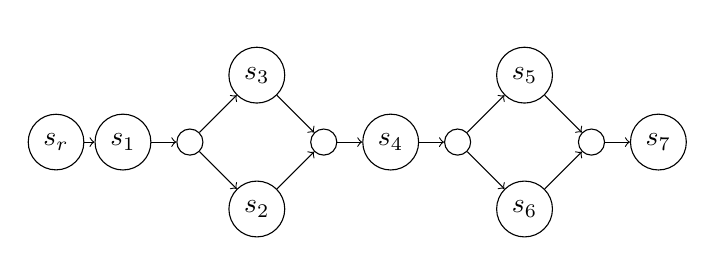
\begin{tikzpicture}[scale=0.85]
    % Nodes
    \node[draw, circle] (node1) at (0,0) {$\s_r$};
    \node[draw, circle] (node2) at (1,0) {$\s_1$};
    \node[draw, circle] (node3) at (2,0) {$\timesOperator$};
    \node[draw, circle] (node4) at (3,-1) {$\s_2$};
    \node[draw, circle] (node5) at (3,1) {$\s_3$};
    \node[draw, circle] (node6) at (4,0) {$\timesOperator$};
    \node[draw, circle] (node65) at (5,0) {$\s_4$};
    \node[draw, circle] (node7) at (6,0) {$\plusOperator$};
    \node[draw, circle] (node8) at (7,1) {$\s_5$};
    \node[draw, circle] (node9) at (7,-1) {$\s_6$};
    \node[draw, circle] (node10) at (8,0) {$\plusOperator$};
    \node[draw, circle] (node11) at (9,0) {$\s_7$};
    % Text on top
    \node[above] at (node1.north) { $\fChartFunction$};
    \node[above] at (node2.north) { $\fChartFunction$};
    \node[above] at (node3.north) {};
    \node[above] at (node4.north) { $\fChartFunction$};
    \node[above] at (node5.north) { $\fChartFunction$};
    \node[above] at (node65.north) { $\fChartFunction$};
    \node[above] at (node8.north) { $\fChartFunction$};
    \node[above] at (node9.north) { $\fChartFunction$};
    \node[above] at (node11.north) { $\fChartFunction$};
    % Connection
    \draw[->] (node1) -- (node2);
    \draw[->] (node2) -- (node3);
    \draw[->] (node3) -- (node4);
    \draw[->] (node3) -- (node5);
    \draw[->] (node5) -- (node6);
    \draw[->] (node4) -- (node6);
    \draw[->] (node6) -- (node65);
    \draw[->] (node65) -- (node7);
    \draw[->] (node7) -- (node8);
    \draw[->] (node7) -- (node9);
    \draw[->] (node8) -- (node10);
    \draw[->] (node9) -- (node10);
    \draw[->] (node10) -- (node11);
  \end{tikzpicture}
  \caption{Service flow}
  \label{fig:service_flow}
\end{figure}
\begin{definition}[Service Flow] \label{def:service_flow}
  A Service Flow S(\V,\E,$\fChartFunction$), is a direct acyclic graph having a root \vi{r}$\in$\V, a vertex \vi{i}$\in$\V\ for each service $s_i$,
  two additional vertices \vi{c},\vi{m}$\in$\V$_{\timesOperator}$$\subset$\V\ for each alternative ($\timesOperator$) structure modeling the alternative execution (\emph{choice}) of operations and the retrieval (\emph{merge}) of the results,
        respectively, and two additional vertices \vi{f},\vi{j}$\in$\V$_{\plusOperator}$$\subset$\V\ for each parallel ($\plusOperator$) structure modeling the contemporary execution (\emph{fork}) of operations and the integration (\emph{join}) of their results, respectively. \TP\,is an annotation function, assigning to each vertex \vi{i}$\in$\V\ a transformation function \TP.
\end{definition}
% \begin{definition}[Big Data Analytics Pipeline] \label{def:pipeline}
%   A Big Data Analytics pipeline \G(\V,\E) is a direct acyclic graph having a root \vi{r}$\fn$\V, a vertex \vi{i}$\fn$\V$_I$$\subseteq$\V\ for each job \job{i} invocation, two additional vertices \vi{c},\vi{m}$\fn$\V$_{\otimes}$$\subset$\V\ for each alternative ($\otimes$) structure modeling the alternative execution (\emph{choice}) of operations and the retrieval (\emph{merge}) of the results,
%     respectively, and two additional vertices \vi{f},\vi{j}$\fn$\V$_{\oplus}$$\subset$\V\ for each parallel ($\oplus$) structure modeling the contemporary execution (\emph{fork}) of operations and the integration (\emph{join}) of their results, respectively.
% \end{definition}

% We note that each vertex \vi{i} model a job \job{i} provided by an organization \org{i}.
% We also note that an analytics pipeline can be deployed following a centralized or a decentralized approach as discussed in detail in Section \ref{sec:architecture}.

% \begin{figure}[!t]
%   \fncludegraphics[width=0.98\columnwidth]{generaleFig1.pdf}
%   \caption{Big Data Analytics pipeline graphs with a coalition of organization for a given processing lineage.}\label{fig:BDpipeline}
% \end{figure}

%

%Solid arrows present the typical batch or analytics model generation flows. Dashed arrows present typical streaming or prediction flows. \CH{togliere dalla figura la linea che separa le due procedure e le scritte ingestion procedure e analytics procedure?}
%The coalition creation is driven by missions including emergency and disaster management, humanitarian operations, or simply interdependent organizations.



\section{Service Template}\label{sec:service_template}
The main point of our investigation is a service-based environment where services are combined strategically with policies that cater to the specific needs of the user.

The service template enhances the service flow defined in \cref{sec:service_definition}, incorporating a policy function to each service.
The policy function serves as a tag to select services within the framework.
This approach allows for the elimination of services that do not meet the user's data treatment requirements.
In addition, the policy directs the system on the necessary data transformations before entering a service.


At the crux of effective service composition lies the pivotal role played by the service template.
Functioning as a high-level composition of services labeled with predefined policies,
the service template serves as a structured blueprint facilitating the decision-making process for the  \user.
\begin{definition}[Service Template] \label{def:pipeline}
  A Service Template \T(\V,\E,$\iChartFunction{}$), is a direct acyclic graph having a root \vi{r}$\in$\V, a vertex \vi{i}$\in$\V\ for each service $s_i$,
  two additional vertices \vi{c},\vi{m}$\in$\V$_{\timesOperator}$$\subset$\V\ for each alternative ($\timesOperator$) structure modeling the alternative execution (\emph{choice}) of operations and the retrieval (\emph{merge}) of the results,
        respectively, and two additional vertices \vi{f},\vi{j}$\in$\V$_{\plusOperator}$$\subset$\V\ for each parallel ($\plusOperator$) structure modeling the contemporary execution (\emph{fork}) of operations and the integration (\emph{join}) of their results, respectively. $\iChartFunction{}$ is an annotation function, assigning to each vertex \vi{i}$\in$\V\ a set of policies \Pset{i}.
\end{definition}


% More detail about the structure modeling the alternative and parallel follows :

% \textbf{Sequence} ($\plusOperator$). It composes two service, $wsi$ and $wsj$, in a sequence. $wsi\plusOperator wsj$ mimics a composition where $wsj$ is executed after $wsi$.

% \textbf{Alternative} ($\timesOperator$). It composes two service, $wsi$ and $wsj$, in an alternative. $wsi\timesOperator wsj$ mimics a composition where either $wsi$ or $wsj$ is executed.

% \textbf{Parallel} ($\plusOperator$). It composes two service, $wsi$ and $wsj$, in parallel. $wsi\plusOperator wsj$ mimics a composition where both $wsi$ and $wsj$ are executed simultaneously.
\begin{figure}[ht!]
  \centering
  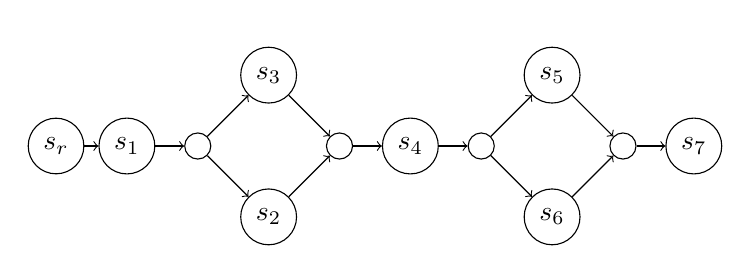
\begin{tikzpicture}[scale=0.9]
    % Nodes
    \node[draw, circle] (node1) at (0,0) {$\s_r$};
    \node[draw, circle] (node2) at (1,0) {$\s_1$};
    \node[draw, circle] (node3) at (2,0) {$\timesOperator$};
    \node[draw, circle] (node4) at (3,-1) {$\s_2$};
    \node[draw, circle] (node5) at (3,1) {$\s_3$};
    \node[draw, circle] (node6) at (4,0) {$\timesOperator$};
    \node[draw, circle] (node65) at (5,0) {$\s_4$};
    \node[draw, circle] (node7) at (6,0) {$\plusOperator$};
    \node[draw, circle] (node8) at (7,1) {$\s_5$};
    \node[draw, circle] (node9) at (7,-1) {$\s_6$};
    \node[draw, circle] (node10) at (8,0) {$\plusOperator$};
    \node[draw, circle] (node11) at (9,0) {$\s_7$};
    % Text on top
    \node[above] at (node1.north)  {$\tChartFunction$};
    \node[above] at (node2.north)  {$\tChartFunction$};
    \node[above] at (node3.north)  {                 };
    \node[above] at (node4.north)  {$\tChartFunction$};
    \node[above] at (node5.north)  {$\tChartFunction$};
    \node[above] at (node65.north) {$\tChartFunction$};
    \node[above] at (node8.north)  {$\tChartFunction$};
    \node[above] at (node9.north)  {$\tChartFunction$};
    \node[above] at (node11.north) {$\tChartFunction$};
    % Connection
    \draw[->] (node1) -- (node2);
    \draw[->] (node2) -- (node3);
    \draw[->] (node3) -- (node4);
    \draw[->] (node3) -- (node5);
    \draw[->] (node5) -- (node6);
    \draw[->] (node4) -- (node6);
    \draw[->] (node6) -- (node65);
    \draw[->] (node65) -- (node7);
    \draw[->] (node7) -- (node8);
    \draw[->] (node7) -- (node9);
    \draw[->] (node8) -- (node10);
    \draw[->] (node9) -- (node10);
    \draw[->] (node10) -- (node11);
  \end{tikzpicture}
  \caption{Service composition template}
  \label{fig:service_composition_template}
\end{figure}

\subsection{Policy}
% \subsubsection{Annotations}
% \subsubsection{Transformation}
The access control language proposed in this paper is taken from our previous work in \cite{}.
It extends an attribute-based access control model that offers flexible fine-grained authorization capabilities and exploits XACML \cite{XACML} obligations to introduce preemptive data transformations.
Indeed, in a collaborative big data scenario, preemptive data transformations are more suitable than denying access to data.
For this reason, when a subject makes an access request to a resource, our access control filters the set of results according to the subject's privileges, obtaining data protection by removing or obfuscating sensitive attributes rather than denying access to full data.

We tailor the common key elements of an attribute-based access control model to deal with the peculiarities of a big data scenario.
The access control policy expresses access conditions based on key elements and their attributes as follows.

\begin{definition}[Policy Condition]\label{def:policy_cond}
  A \emph{Policy Condition} is a Boolean expression of the form $($\emph{attr\_name} op \emph{attr\_value}$)$, with op$\in$\{$<$,$>$,$=$,$\neq$,$\leq$,$\geq$\}, \emph{attr\_name} an attribute label, and \emph{attr\_value} the corresponding attribute value.
\end{definition}

A policy is then defined as follows.

\begin{definition}[Policy]\label{def:policy_rule}
  A {\it policy P} is 5-uple $<$\textit{subj}, \textit{obj}, \textit{action}, \textit{env}, \textit{datatrans}$>$, where:
  \begin{itemize}
    \item Subject \textit{subj} defines a user or the service provider of a job issuing access requests to perform operations on objects. It is of the form $<$\emph{id}, \emph{PC}$>$, where \emph{id} defines a class of users (e.g., policeman), and \emph{PC} is a set of \emph{Policy Conditions} on the subject, as defined in Definition \ref{def:policy_cond}. For instance, $<$\emph{user},\{(age $\geq$ 18)\}$>$ refers to a person of legal age.

    \item Object \textit{obj} defines any data whose access is governed by the policy. It is of the form $<$\emph{type}, \emph{PC}$>$, where: \emph{type} defines the type of object, such as a file (e.g., a video, text file, image, etc.), a SQL or noSQL database, a table, a column, a row, or a cell of a table, and \emph{PC} is a set of \emph{Policy Conditions} defined on the object's attributes. For instance, $<$\emph{file},\{(creation\_date $<$ 2020/12/05)\}$>$ refers to a file created before 2020/12/05.

    \item Action \textit{action} defines any operations that can be performed within a big data environment, from traditional atomic operations on databases (e.g, CRUD operations varying depending on the data model) to coarser operations, such as an Apache Spark Direct Acyclic Graph (DAG), an Hadoop MapReduce, an analytics function call, or an analytics pipeline.

    \item Environment \textit{env} defines a set of conditions on contextual attributes, such as time of the day, location, IP address, risk level, weather condition, holiday/workday, emergency. It is a set \emph{PC} of
          \emph{Policy Conditions} as defined in Definition \ref{def:policy_cond}.
          For instance, \{(weather\_conditions $=$ red\_alert)\} refers to a red alert broadcasted for weather conditions.

    \item Data Transformation \textit{datatrans} defines a set of security and privacy-aware transformations on \textit{obj}, focusing on compliance to regulations and standards, in addition to simple format conversions.
  \end{itemize}
\end{definition}

\subsubsection{Policy Decision/Policy Matching}
\subsubsection{Policy Enforcement}
\subsubsection{Policy Evaluation}
\section{Service Instance}

\begin{figure}[ht!]
  \centering
  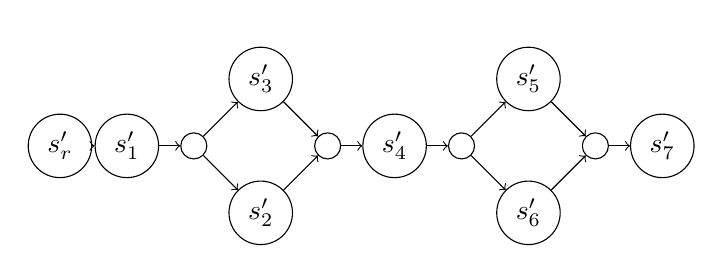
\begin{tikzpicture}[scale=0.85]
    \node[draw, circle] (node1) at (0,0) {$\s^\prime_r$};
    \node[draw, circle] (node2) at (1,0) {$\s^\prime_1$};
    \node[draw, circle] (node3) at (2,0) {$\timesOperator$};
    \node[draw, circle] (node4) at (3,-1) {$\s^\prime_2$};
    \node[draw, circle] (node5) at (3,1) {$s^\prime_3$};
    \node[draw, circle] (node6) at (4,0) {$\timesOperator$};
    \node[draw, circle] (node65) at (5,0) {$\s^\prime_4$};
    \node[draw, circle] (node7) at (6,0) {$\plusOperator$};
    \node[draw, circle] (node8) at (7,1) {$\s^\prime_5$};
    \node[draw, circle] (node9) at (7,-1) {$\s^\prime_6$};
    \node[draw, circle] (node10) at (8,0) {$\plusOperator$};
    \node[draw, circle] (node11) at (9,0) {$\s^\prime_7$};
    % Text on top
    \node[above] at (node1.north) { \footnotesize$\iChartFunction$};
    \node[above] at (node2.north) { \footnotesize$\iChartFunction$};
    \node[above] at (node3.north) {};
    \node[above] at (node4.north) { \footnotesize$\iChartFunction$};
    \node[above] at (node5.north) { \footnotesize$\iChartFunction$};
    \node[above] at (node65.north) { \footnotesize$\iChartFunction$};
    \node[above] at (node8.north) { \footnotesize$\iChartFunction$};
    \node[above] at (node9.north) { \footnotesize$\iChartFunction$};
    \node[above] at (node11.north) { \footnotesize$\iChartFunction$};
    % Connection
    \draw[->] (node1) -- (node2);
    \draw[->] (node2) -- (node3);
    \draw[->] (node3) -- (node4);
    \draw[->] (node3) -- (node5);
    \draw[->] (node5) -- (node6);
    \draw[->] (node4) -- (node6);
    \draw[->] (node6) -- (node65);
    \draw[->] (node65) -- (node7);
    \draw[->] (node7) -- (node8);
    \draw[->] (node7) -- (node9);
    \draw[->] (node8) -- (node10);
    \draw[->] (node9) -- (node10);
    \draw[->] (node10) -- (node11);
  \end{tikzpicture}
  \caption{Service composition instance}
  \label{fig:service_composition_instance}
\end{figure}




% \textbf{Loop} ($\oslash$). It composes a service composition by iteratively executing the same composition. $\oslash wsi$ mimics a composition where the service $wsi$ is executed a given number of times. In the following, $\oslash$ is considered as a sequence of $\oslash$ services with the same composition $wsi$.

% \textbf{Containment} ($\tau$). It composes two service, $wsi$ and $wsj$, in a containment relation. $wsi\tau wsj$ mimics a basic composition pattern where $wsj$ is called within $wsi$, meaning that $wsi$ assumes the role of a container and $wsj$ uses container-level functionalities (e.g., signature, encryption) to secure the message exchange. We note that the containment operator does not have a direct mapping to BPEL constructs because it is applied to a specific service before the BPEL process is even considered.
\subsection{Instance}
When the template is filled with the necessary services, it becomes an instance that reflects the actual implementation of those services. This instance follows the same flow as the template, but with the added function F that represents the transformation operations carried out by the service.

Let \T(\V,\E,$\iChartFunction$) be a Service Template, a Composite Service instance is \T'(\V',\E,$\iChartFunction$,$\gamma$) is a directed acyclic graph where:
$s_r=s'_r$, for each vertex \vi{}$\in$\V$_{\timesOperator}$$\cup$\V$_{\plusOperator}$ it exists a corresponding vertex \vi{}'$\in$\V'$_{\timesOperator}$$\cup$\V'$_{\plusOperator}$,
    and for each \vi{i}$\in$ \V\ it exists a corresponding \vi'{i}$\in$ \V'\ instantiated with a real service \vi{i} having a policy \Pset{i}, such that the following conditions hold:
    \begin{itemize}
      \item $s_i$ satisfies functional requirements in $G_{\iChartFunction}(V,E,\iChartFunction)$.
      \item \Pset{i} satisfies $\iChartFunction(v_i)$.
    \end{itemize}

    The Composite Service  instance  is generated by traversing the Service Template with a breadth-first search algorithm,
    starting from the root vertex \vi{r}. Then for each vertex \vi{i} in the Service Template, the corresponding vertex \vi{i}'$\in$ \V'\ is generated.
    Finally for each vertex  \vi{i}'$\in$ \V'\ a two step selection approach is applied as follows.
\begin{itemize}
  \item \textit{Selection Algorithm} - It matches requirements in $\iChartFunction$ with the policy $\iChartFunction$, and returns a set of services $S_i$ that satisfy the requirements.
  \item \textit{Comparison Algorithm} - Upon retrieving a set of compatible services, it produces a ranking of these services according their scoring function.
        The scoring function is calculated according some metrics, which evaluate the quality of the data resulting from the service execution.
        More details about the metrics are provided in Section \ref{sec:metrics}.
\end{itemize}


% \begin{figure}[H]
%   \centering

%   \begin{tikzpicture}
%     % Nodes
%     \node[draw, circle, minimum size=0.4cm, draw=gray, text opacity=0.5] (node11) at (0,1.2) {Sx};
%     \node[draw, circle, minimum size=1cm] (node1) at (0,0) {S1};
%     \node[draw, circle, minimum size=0.4cm, draw=gray, text opacity=0.5] (node10) at (0,-1.2) {Sy};

%     \node[draw, circle, minimum size=0.4cm, draw=gray, text opacity=0.5] (node22) at (2,1.2) {Sx};
%     \node[draw, circle, minimum size=1cm] (node2) at (2,0) {S2};
%     \node[draw, circle, minimum size=0.4cm, draw=gray, text opacity=0.5] (node21) at (2,-1.2) {Sy};

%     \node[draw, circle, minimum size=1cm] (node3) at (4,0) {$\timesOperator$};

%     \node[draw, circle, minimum size=0.4cm, draw=gray, text opacity=0.5] (node42) at (5,-1.5) {Sx};
%     \node[draw, circle, minimum size=1cm] (node4) at (6,-1.5) {S3};
%     \node[draw, circle, minimum size=0.4cm, draw=gray, text opacity=0.5] (node41) at (7,-1.5) {Sy};

%     \node[draw, circle, minimum size=1cm] (node5) at (6,1.5) {S4};
%     \node[draw, circle, minimum size=0.4cm, draw=gray, text opacity=0.5] (node51) at (5,1.5) {Sx};
%     \node[draw, circle, minimum size=0.4cm, draw=gray, text opacity=0.5] (node52) at (7,1.5) {Sy};
%     % Connection
%     \draw[->] (node1) -- (node2);
%     \draw[->] (node2) -- (node3);
%     \draw[->] (node3) -- (node4);
%     \draw[->] (node3) -- (node5);
%   \end{tikzpicture}
%   \caption{Service composition instance}
%   \label{fig:service_composition_instance}
% \end{figure}
% \[ \forall S \in \mathrm{S}_{C}  \exists  \iChartFunction(S) = \mathrm{S}_{1} \]


\begin{figure}
  \centering
  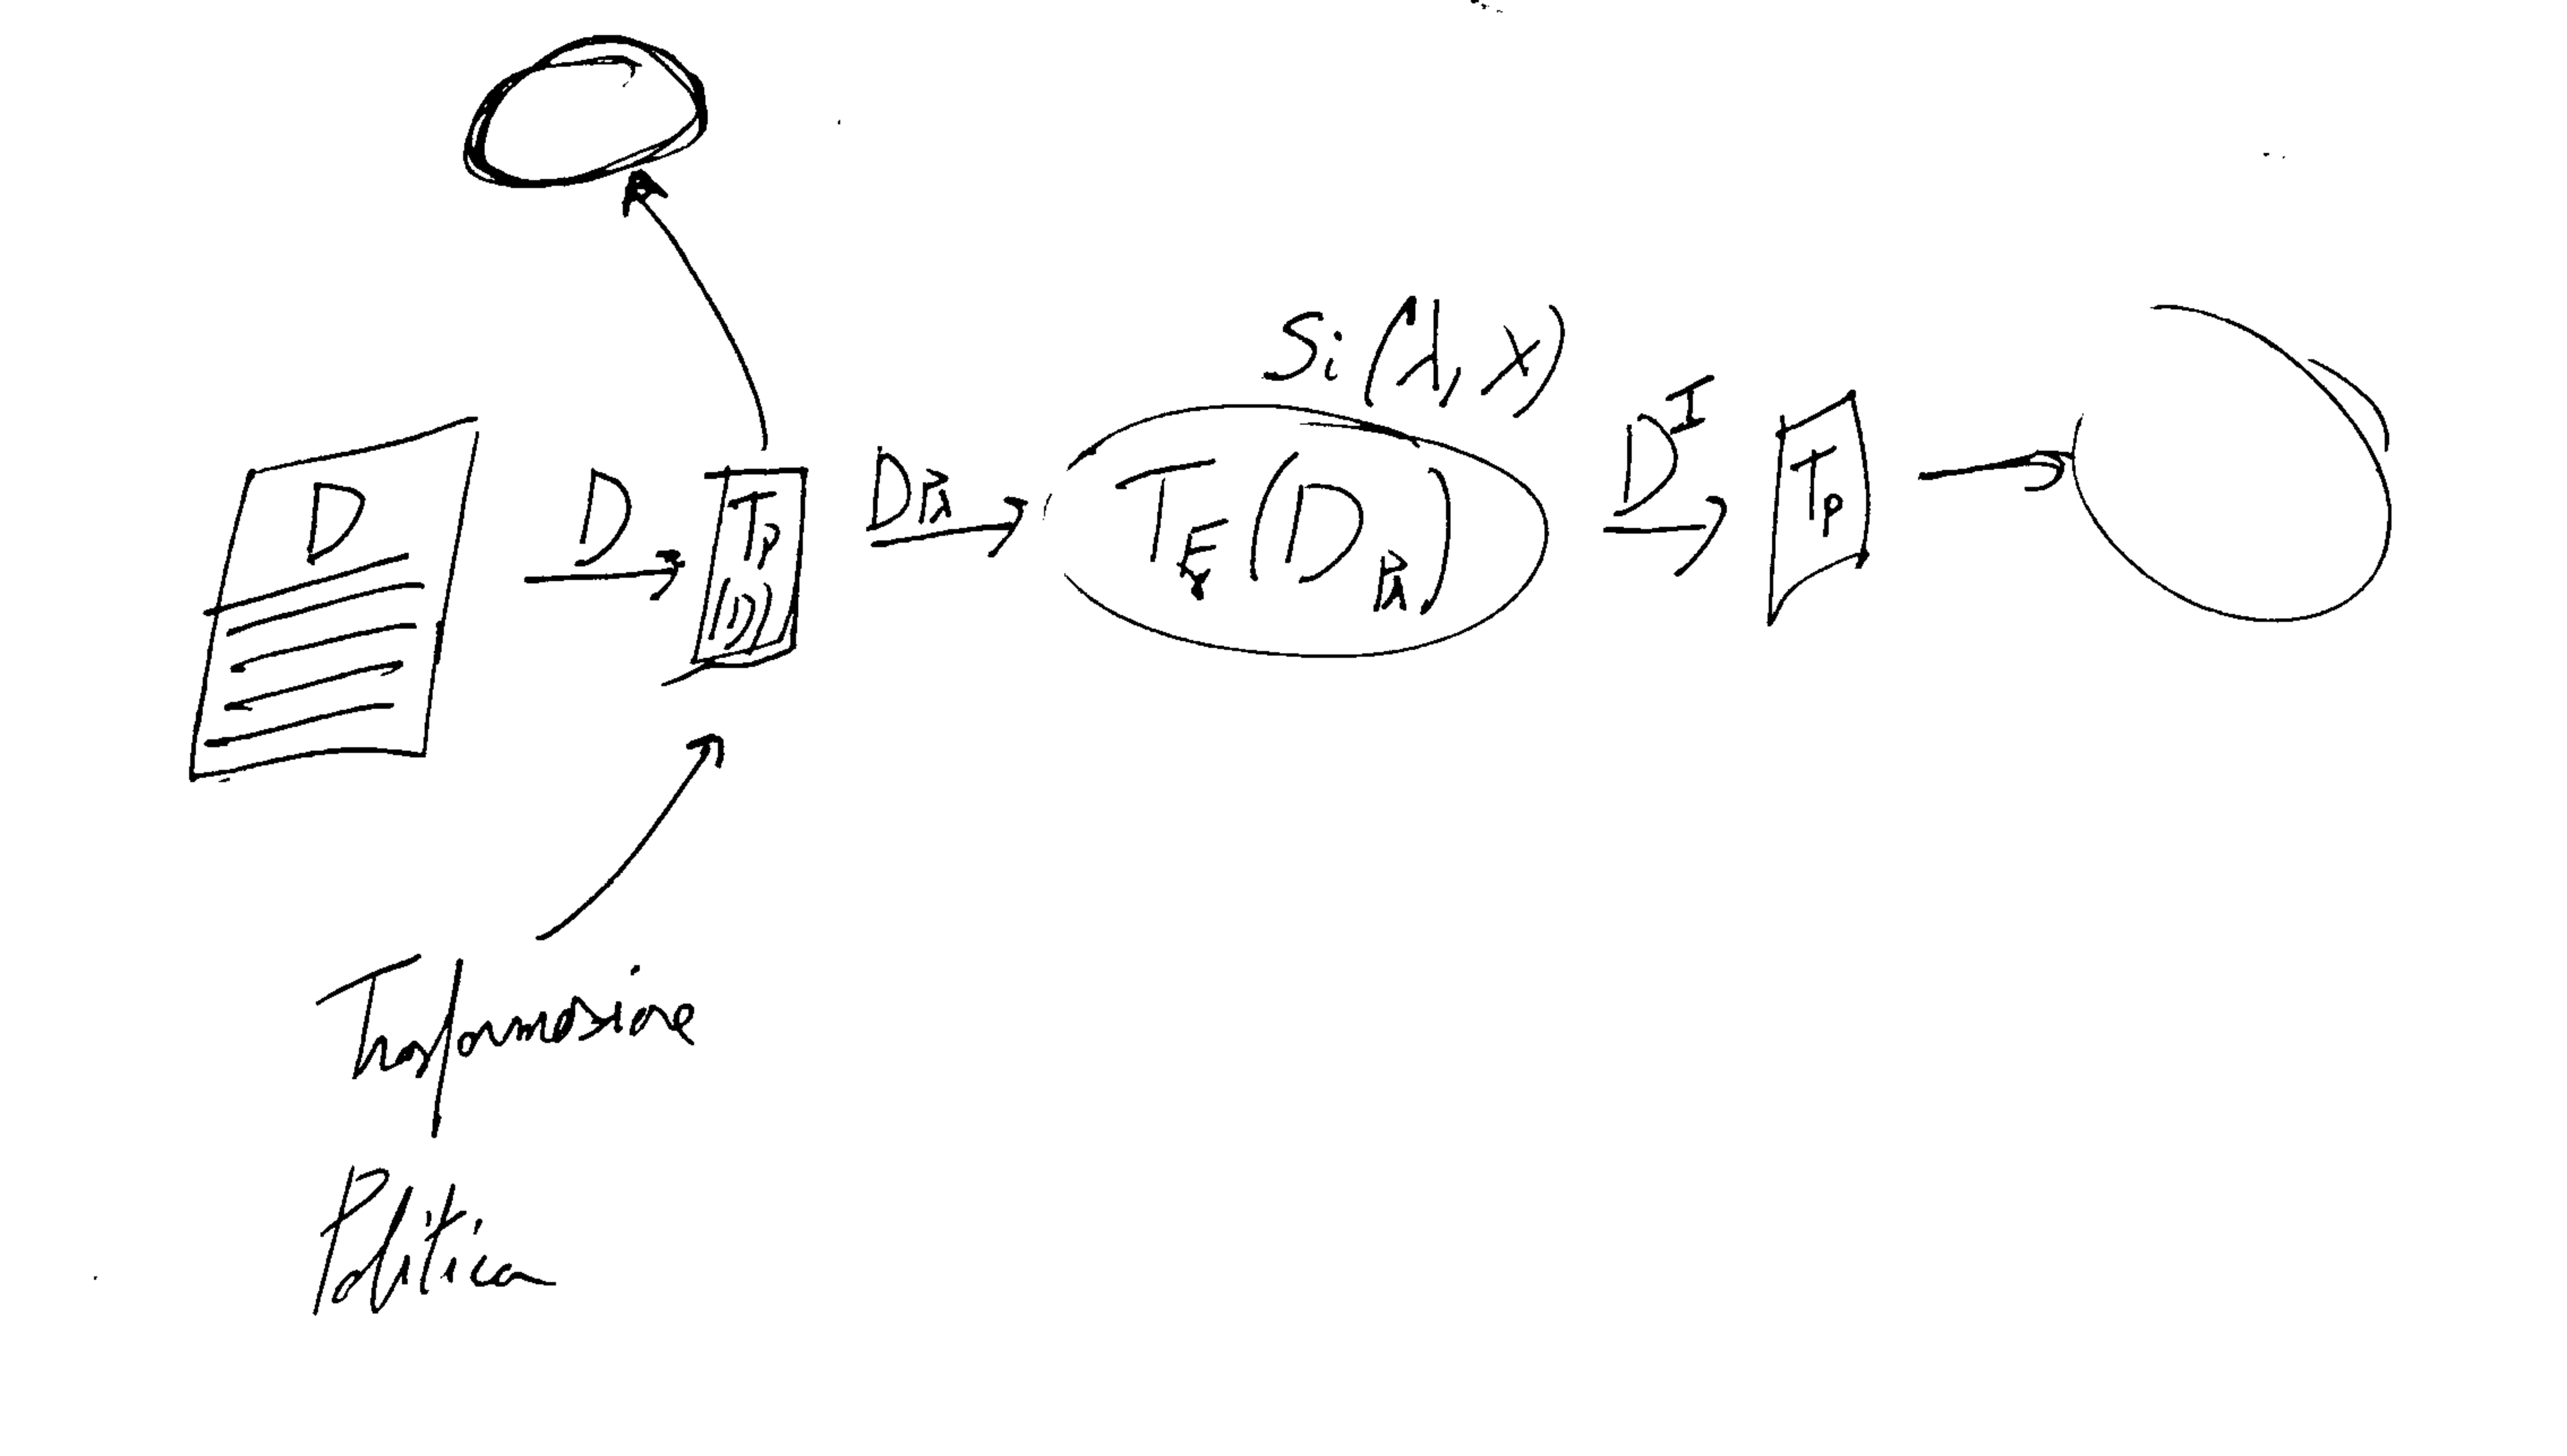
\includegraphics[width=\columnwidth]{serviceDetail.pdf}
  \caption{Service Detail}
  \label{fig:service_detail}
\end{figure}